\documentclass[12pt]{article}
\usepackage[dvipsnames]{xcolor}
\usepackage{hyperref, pagecolor, mdframed }
\usepackage{graphicx, amsmath, latexsym, amsfonts, amssymb, amsthm,
amscd, geometry, xspace, enumerate, mathtools}
\usepackage{tikz}

\newcommand{\fdiv}{\textrm{div}}
\newcommand{\Z}{\mathbb{Z}}
\newcommand{\Q}{\mathbb{Q}}
\newcommand{\K}{\mathbb{K}}
\newcommand{\algK}{\overline{K}}
\newcommand{\algF}{\overline{\mathbb{F}}}
\newcommand{\Pic}{\textrm{Pic}}
\newcommand{\Hom}{\textrm{Hom}}

\hypersetup{
    colorlinks=true,
    linkcolor=blue,
    urlcolor=Green,
    filecolor=RoyalPurple
}

\definecolor{wgrey}{RGB}{148, 38, 55}
\title{L'isogenie duale}
\date{8 juillet 2023}
\begin{document}
%\tableofcontents
\maketitle

\noindent \noindent \textbf{Petit rappel} : Sur la courbe elliptique $E$, $D\in Div^0(E)$ est principal ssi 
\begin{itemize}
    \item deg$(D)=0$
    \item Si $D=\sum n_i(P_i)$, $\sum [n_i]P_i=O$ dans $E$.
\end{itemize}    

\noindent \textbf{\color{wgrey} La def :} Pour $\phi~:~E_1\rightarrow E_2$ on considère \\\begin{center}
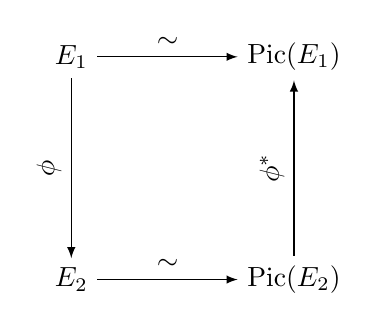
\begin{tikzpicture}[x=1cm,y=1cm, >=latex, ->]
    \node(0) at (135 : 2) {$E_1$};
    \node(1) at (45 : 2) {$\Pic(E_1)$};
    \node(2) at (-135 : 2) {$E_2$};
    \node(3) at (-45 : 2) {$\Pic(E_2)$};

    \foreach \k/\l in {0/1, 2/3}{\draw(\k)--(\l) node[midway, above]{$\sim$};}
    \draw(3)--(1) node[midway, above, sloped]{$\phi^*$};
    \draw(0)--(2) node[midway, below, sloped]{$\phi$};
\end{tikzpicture}

(où les $\tau_i~:~E_i\rightarrow \Pic(E_i)$ sont données par $P\mapsto (P)-(O)$.)

\end{center}
Alors $\hat{\phi}$ est donnée par $\hat{\phi}(Q)=\tau_1^{-1}(\phi^*(Q)-\phi^*(O))$.


\end{document}
